% !TEX root =  ../../thesis.tex

\chapter{Analysis of blood donor data set}
\label{ch : blood_donor}
 
 In this chapter we have presented the analysis of the blood donor data set \citep{nasserinejad_prevalence_2015} using the Bayesian heterogeneity model. The data set consists of 1595 male blood donors who donated blood multiple times over a period of many years. On each visit to the donation center, the following information was noted: Season in which blood was donated (Cold/Hot), Volume of blood donated (ml), age at the time of donation (years), a binary indicator Donate (yes/no) specifying if the donor was allowed to donate the blood, Hemoglobin (Hb) of the patient at the time of donation, and the date of visit. Other variables derived from date of visit such as time since previous donation (TSPD), time since previous visit (TSPV) were also present in the data set. \citet{nasserinejad_predicting_2013,nasserinejad_prevalence_2015,nasserinejad_prediction_2016} have analyzed this data set extensively using transition models, mixed models, growth mixture models and latent class mixed effects transition models. The analysis was used to predict the Hb level of donors so that they are invited for donation at an optimal time, i.e. when their Hb levels are not too low because of the previous donations and other factors.\\

 For the purpose of this thesis we did not use the entire data set of 1595 patients as Bayesian computation for heterogeneity model using the entire data set required large amount of computational resources. Instead we used a simple random sample of the data consisting of 250 subjects.

\section{Motivation for analysis with Bayesian heterogeneity model}
 In the analysis using growth mixture models \citet{nasserinejad_prevalence_2015} found 4 different underlying subpopulations in the data set. Firstly, those which had a relatively stable Hb level over donations. Secondly, those which had a higher baseline Hb level than those in category 1 and also showed a slow decline of Hb level over donations. Thirdly, those which showed a moderately sharp decline in Hb level over donations, and lastly those which showed a steep decline in Hb levels despite beginning at high initial Hb levels. Because of the presence of different subpopulations, a single methodology to decide the time of next blood donation for subjects from all subpopulations may not be effective. The aim of applying the Bayesian heterogeneity model to this dataset was to provide an alternative modeling framework for such data sets.

\section{Frequentist analysis}
\label{sec : frequentist_blood_donor}
We began with a frequentist analysis of the blood donor data set to select the right mean structure for our models ahead. This was necessary because omitting a required covariate in the mean structure could lead to incorrect estimates of the covariance matrix. Secondly, a frequentist analysis provided us good starting values for the various parameters in our model. Thirdly we also wanted check if the Bayesian analysis results were consistent with the frequentist analysis results. For the random effects structure we considered a model with both random intercept and random slope. For the choice of random slope we selected the variable 'number of donations in last 2 years' because that was deemed as a suitable variable for random slope by \citet{nasserinejad_prevalence_2015}. For selecting the mean structure we did F-tests and likelihood ratio tests based on ML. We found the following mean structure to be suitable.

\begin{equation}
\label{eq : blood_donor_model}
\begin{split}
\boldsymbol{y}_{ij} = \beta_0 + \beta_1*\text{Age}_{ij} + \beta_2*\text{Season}_{ij} + \beta_3*\text{Donate}_{ij} + \beta_4*\text{TSPD}_{ij}\\
+ \beta_4*\text{\#donationLast2Years}_{ij} + \beta_5*\text{\#donationLast2Years}_{ij}*\text{TSPD}_{ij}\\
+ \beta_6*\text{\#donationLast2Years}_{ij}*\text{Donate}_{ij} + \beta_7*\text{\#donationLast2Years}_{ij}^2\\
+ b_0 + b_1 * \text{\#donationLast2Years}_{ij} + \varepsilon_{ij}
\end{split}
\end{equation}

where, Age and TSPD have been standardized to have mean 0 and variance 1, $\text{\#donationLast2Years}_{ij}$ have been downscaled by a factor of 100 so that the random slope variance scale is upscaled. Similarly the intercept we used was 0.1, thus upscaling the random intercept variance. It is important to note that this model assumes a single multivariate normal distribution for the distribution of random effects. Table \ref{table : frequentist_fixed effects} shows the parameter estimates for this model. 

\begin{table}[!htb]
\centering
\captionsetup{justification=centering}
\caption{Frequentist fixed effect estimates and random variance estimates for model \ref{eq : blood_donor_model}. REML was used for obtaining these parameter estimates.}
\label{table : frequentist_fixed effects}
\begin{tabular}{@{}lrr@{}}
\toprule
Fixed Effects ($\beta$) & Mean & Standard Error \\ \midrule
intercept & 94.121 & 0.429 \\
Age & -0.086 & 0.026 \\
\#donationLast2Years & -7.265 & 1.555 \\
TSPD & -0.036 & 0.015 \\
Season (Hot) & -0.080 & 0.016 \\
Donate (TRUE) & 0.155 & 0.037 \\
\#donationLast2Years * TSPD & 0.020 & 0.006 \\
\#donationLast2Years * Donate & 4.689 & 0.995 \\
$\text{\#donationLast2Years}^2$ & -52.796 & 15.237 \\ \bottomrule
\end{tabular}

\begin{tabular}{@{}lr@{}}
\toprule
Covariance Parameters & Estimate \\ \midrule
$\sigma^2_\text{Intercept}$ & 19.971 \\
$\sigma_\text{Intercept, Slope}$ & -14.266 \\
$\sigma^2_\text{Slope}$ & 40.183 \\
$\sigma^2$ & 0.201 \\ \bottomrule
\end{tabular}
\end{table}

\section{Bayesian analysis}
\label{sec : blood_donor_bayesian_analysis}
We next extended the model in equation \ref{eq : blood_donor_model} for fitting the Bayesian version of the Heterogeneity model proposed by \citet{verbeke_linear_1996}. Since the random component in the Bayesian heterogeneity model follows a mixture distribution we fitted mixtures of 1 to 5 components. We removed the intercept and the fixed effect of number of donations in last 2 years from the model to impose hierarchical centering on the random effects. The next step we took for model fitting was generating a plot of random part of the model in \ref{eq : blood_donor_model} using the approach mentioned in \ref{subsec : ds_description}. The corresponding plot shown in figure \ref{fig : rough_idea_blood_donor} shows that there could be perhaps 1 component, or if there are more then the components are not well separated. We saw in the case of data set 5 (figure \ref{fig : ds_3fused3ppg_randplot}) which also had fused components, that we required a slightly higher value for the hyperparameter of the Dirichlet prior for weight distribution. Thus we tested $\text{Dir}(1, 1,...1)$, $\text{Dir}(2, 2,...2)$ and $\text{Dir}(3, 3,...3)$ for the blood donor data set. From the various simulations we ran we found that $\text{Dir}(2, 2,...2)$ prior gave the same results as Dirichlet priors with slightly higher values of the hyperparameters and so we stuck with it. As for the length of MCMC chains, we ran 500,000 iterations with a thinning of 150 and a burn in of 100,000 iterations.\\

\begin{figure}
	\centering
	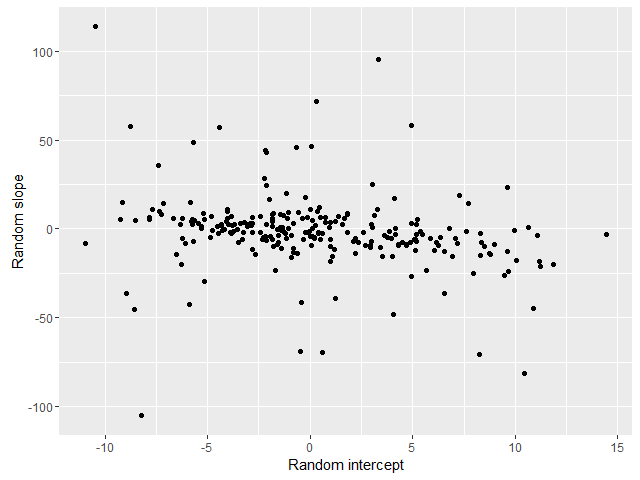
\includegraphics[scale=0.5]{mainmatter/chapter_6_blood_donor/rough_estimate_random_effects.png}
	\caption{Rough estimate $\tilde{\boldsymbol{b}_i}$ for random effects}
	\label{fig : rough_idea_blood_donor}
\end{figure}

The first model we fitted was without any mixture of random effects. The parameter estimates we obtained from this model are shown in table \ref{table : bayesian fixed effects}. It is quite clear from these results that the Bayesian results are almost the same as the frequentist estimates.

\begin{table}[!htb]
\centering
\captionsetup{justification=centering}
\caption{Bayesian fixed effect estimates and random effect estimates for model \ref{eq : blood_donor_model}. The intercept and \#donationLast2Years have been removed for hierarchical centering.}
\label{table : bayesian fixed effects}
\begin{tabular}{@{}lrrr@{}}
\toprule
Fixed Effects ($\beta$) & Mean & Median & 95\% HPDI \\ \midrule
Age & -0.086 & -0.086 & -0.135, -0.034\\
TSPD & -0.037 & -0.037 & -0.068, -0.009 \\
Season (Hot) & -0.080 & -0.080 & -0.109, -0.048\\
Donate (TRUE) & 0.157 & 0.157 & 0.083, 0.232 \\
\#donationLast2Years * TSPD & 0.020 & 0.020 & 0.009, 0.031  \\
\#donationLast2Years * Donate & 4.694 & 4.715 & 2.492, 6.492 \\
$\text{\#donationLast2Years}^2$ & -50.247 & -50.449 & -77.843, -21.436 \\ \bottomrule
\end{tabular}

\begin{tabular}{@{}lrrr@{}}
\toprule
Covariance Parameters & Mean & Median & 95\% HPDI \\ \midrule
$b_{\text{Intercept}}^C$& 94.130 & 94.142 & 93.303, 94.954\\
$b_{\text{slope}}^C$ & -7.504 & -7.531 & -10.639, -4.531\\
$\sigma^2_\text{Intercept}$ & 20.098 & 19.883 & 15.784, 24.559\\
$\sigma_\text{Intercept, Slope}$ & -13.989 & -13.771 & -20.879, -7.903\\
$\sigma^2_\text{Slope}$ & 39.396 & 39.061 & 27.895, 53.443\\
$\sigma^2$ & 0.201 & 0.201 & 0.191, 0.213\\ \bottomrule
\end{tabular}
\end{table}

Next we fitted models with 2 to 5 components in the mixture of random effects. In the case of fitting two components to the mixture we applied identifiability constraints on the weights, i.e. $\eta_1 < \eta_2$. Without these constraints we observed label switching and thus the posteriors were bimodal. For 3 or more components however identifiability constraints were not useful. For e.g. in the case of fitting 3 components we observed convergence only in some chains when we increased the hyperparameters for the Dirichlet prior (prior for $\boldsymbol{\eta}$) to 13. Since the prior was not informative we discarded the corresponding results.\\

Nevertheless for each of the resulting MCMC chains we calculated the various definitions of DIC given in section \ref{sec : dic}, the results of which are presented in Table \ref{table : dic_blood_donor}. In the simulation study we had observed that $\text{DIC}_4$ was the most discerning of the DIC's, especially also when the mixture components were not well separated. In the latter case $\text{DIC}_1$, $\text{DIC}_2$ and $\text{DIC}_3$ were not much discerning and in one example (data set 7) $\text{DIC}_1$ did not select the right model. $\text{DIC}_5$ and $\text{DIC}_6$ also did not select the right model when components were not well separated. Thus for the blood donor data set we primarily relied on $\text{DIC}_4$. We could not consider models with 3 or more components because the corresponding chains did not converge. Looking at the results in Table \ref{table : dic_blood_donor} it seemed that a model with 2 components was preferable over a model with no mixture. Lastly, we would like to discuss  the pattern of $\text{DIC}_4$ stabilizing for overfitted components. We did observe it for blood donor data set as well and so it was not specific to the data sets in the simulation study. However, it was as not consistent in the blood donor data set as it was for the simulations study.

\begin{table}[!htb]
\centering
\captionsetup{justification=centering}
\caption{DIC for blood donor data set}
\label{table : dic_blood_donor}
\begin{tabular}{@{}rrrrrrr@{}}
\toprule
\# Components Fitted & $\text{DIC}_1$ & $\text{DIC}_2$ & $\text{DIC}_3$  & $\text{DIC}_4$  & $\text{DIC}_5$  & $\text{DIC}_6$  \\ \midrule
1 comp & 4817 & 4816 & 4818 & 7077 & 7532 & 4353 \\
2 comp & 4808 & 4805 & 4811 & 6956 & 7376 & 4306 \\
3 comp & 4755 & 4825 & 4838 & 7024 & 7406 & 4360 \\
4 comp & 4608 & 4723 & 4814 & 7031 & 7360 & 4332 \\
5 comp & 4461 & 4459 & 4818 & 7031 & 7108 & 4327 \\ \bottomrule
\end{tabular}
\begin{tabular}{@{}rrrrrrr@{}}
\toprule
\# Comp Fitted & ${\text{p}_\text{D}}_1$ & ${\text{p}_\text{D}}_2$ & ${\text{p}_\text{D}}_3$ & ${\text{p}_\text{D}}_4$ & ${\text{p}_\text{D}}_5$ & ${\text{p}_\text{D}}_6$ \\ \midrule
1 comp & 13 & 12 & 15 & 13 & 468 & 302 \\
2 comp & 17 & 16 & 19 & 19 & 439 & 247 \\
3 comp & -55 & -15 & 29 & 5 & 387 & 294 \\
4 comp & -183 & -67 & 23 & 30 & 360 & 272 \\
5 comp & -334 & -336 & 23 & 28 & 104 & 269 \\ \bottomrule
\end{tabular}
\end{table}

\subsection{PPC for blood donor data set}
To further verify if 2 components are the correct number of components we used posterior predictive checks. The PPC which we mentioned in section \ref{subsec : ppc_bhtge} had an interesting property that it worked for overfitted models as well because in overfitted models the chains corresponding to fixed effects converged and only the chains corresponding to parameters of some of the component densities did not. To perform PPC we required a sample of number of donations in last 2 years. Instead of randomly generating them we sampled them from the subjects which were not considered for analysis due to computational restrictions. We then generated random effects from the posterior predictive distribution of random effects. Figure \ref{fig : ppc_blood_donor_3comp} to \ref{fig : ppc_blood_donor_5comp} show the distribution of the test statistic \ref{eq : ppc_test_statistic} for the 5 models we considered. It can be seen that the test statistic has the characteristic skewed distribution due to the posteriors of parameters being almost equal to the priors in case of 3 or more number of components in the mixture (see section \ref{subsec : ppc_bhtge}). Another aspect of the result is that the distribution of the test statistic with posterior predictive data overlaps the distribution of test statistic with the sample data. This shows that the model is well fitted to the data. Lastly the PPP values for the various models are shown in Table \ref{table : ppp_blood_donor}. It can be seen that the PPP values are lowest for model with 2 components. However they are not extreme for the overfitted models, a phenomenon which we also observed and discussed in simulation study results (section \ref{subsec : ppc_simulation}). Based on the results of PPC and DIC both, we decided to choose the model with 2 components in the mixture.

\begin{figure}[!htb]
\centering
\captionsetup{justification=centering}
\begin{subfigure}[b]{0.4\textwidth}
		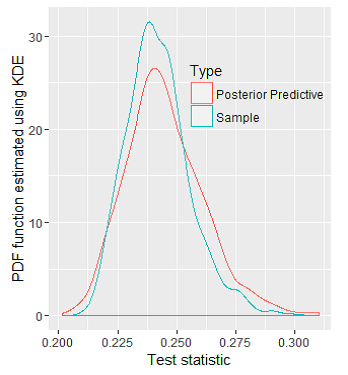
\includegraphics[width=\textwidth]{mainmatter/chapter_6_blood_donor/ppc_1comp.png}
        \caption{\label{fig : ppc_blood_donor_1comp}\#Components fitted = 1}
	\end{subfigure}
	\begin{subfigure}[b]{0.4\textwidth}
		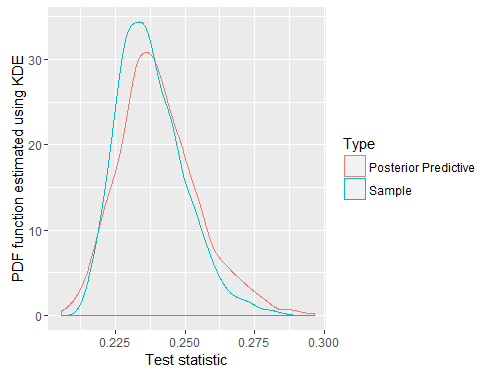
\includegraphics[width=\textwidth]{mainmatter/chapter_6_blood_donor/ppc_2comp.png}	
          \caption{\label{fig : ppc_blood_donor_2comp}\#Components fitted = 2}
	\end{subfigure}
	\caption{PDF function of $T(\boldsymbol{\tilde{r}})$ for underfitted/rightly fitted models applied to the blood donor data set.}
	\label{fig : ppc_blood_donor_underfitted}    
\end{figure} 

\begin{figure}[!htb]
\centering
\captionsetup{justification=centering}
\begin{subfigure}[b]{0.4\textwidth}
		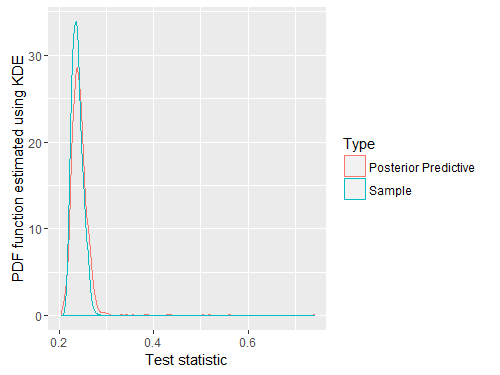
\includegraphics[width=\textwidth]{mainmatter/chapter_6_blood_donor/ppc_3comp.png}	
          \caption{\label{fig : ppc_blood_donor_3comp}\#Components fitted = 3}
	\end{subfigure}
	\begin{subfigure}[b]{0.4\textwidth}
		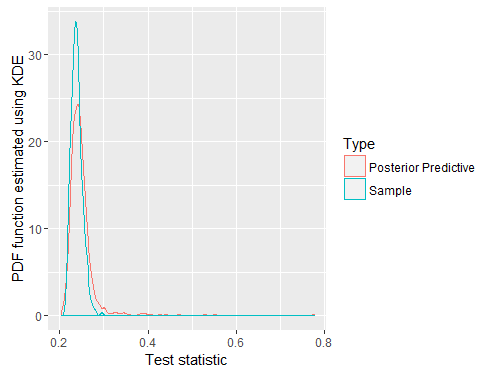
\includegraphics[width=\textwidth]{mainmatter/chapter_6_blood_donor/ppc_4comp.png}	
          \caption{\label{fig : ppc_blood_donor_4comp}\#Components fitted = 4}
	\end{subfigure}
	\begin{subfigure}[b]{0.4\textwidth}
		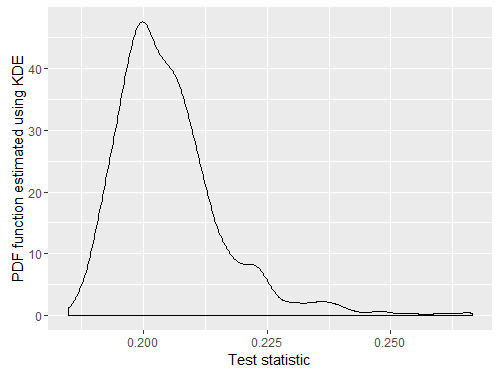
\includegraphics[width=\textwidth]{mainmatter/chapter_6_blood_donor/ppc_5comp.png}	
          \caption{\label{fig : ppc_blood_donor_5comp}\#Components fitted = 5}
	\end{subfigure}
	
	\caption{PDF function of $T(\boldsymbol{\tilde{r}})$ for overfitted models applied to the blood donor data set.}
	\label{fig : ppc_blood_donor_overfitted}    
\end{figure} 

\begin{table}[!htb]
\centering
\captionsetup{justification=centering}
\caption{PPP values for the various models fitted to the blood donor data set.}
\label{table : ppp_blood_donor}
\begin{tabular}{@{}rrrrrrrrr@{}}
\toprule
\# Components fitted & 1 & 2 & 3 & 4 & 5\\ \midrule
PPP Value & 0.619 & 0.591 & 0.677 & 0.701 & 0.758\\ \bottomrule
\end{tabular}
\end{table}

\section{Parameter estimates for the model with 2 components in mixture}
Table \ref{table : bhtge_blooddonor_2comp} shows the parameter estimates for the component densities of the mixture of random effects. Further, figure \ref{fig : eta_blood_donor} to figure \ref{fig : cov_blood_donor} show the posterior densities of the weight distribution $\boldsymbol{\eta}$, location parameters $\boldsymbol{b^C}$ and covariance parameters $\sigma^2_\text{Intercept}$, $\sigma^2_\text{Slope}$, $\sigma_\text{Intercept, Slope}$ which form the covariance matrix $G$. If we consider the mean of the posterior distribution then we can see that the weight distribution ratio for the components is 1:3. Secondly we can see that the posterior densities for location parameters for slope have a slight overlap but that is not the case with random intercept.\\

The first component in the mixture corresponds to the group for which the baseline random component of Hemoglobin is low and and the second component corresponds to the group for which the baseline random component of Hemoglobin is higher. However for the second group the slope is more negative suggesting that relative to group 1 an average subject from group 2 has a more rapid decrease in Hemoglobin levels with frequent donations. Lastly, within group 2 a person who begins with a higher baseline Hemoglobin level, is likely to have a more rapid decrease in Hemoglobin levels with donations. However within group 1 such intra subject difference cannot be generalized because 95\% HPDI for the correlation between random intercept and random slope is [-0.847, 0.980].

\begin{table}[htb]
\centering
\captionsetup{justification=centering}
\caption{Bayesian parameter estimates for the model with 2 components in the mixture of random effects, applied to the Blood donor data set.}
\label{table : bhtge_blooddonor_2comp}
\begin{tabular}{@{}lrrr@{}}
\toprule
Fixed Effects ($\beta$) & Mean & Median & 95\% HPDI \\ \midrule
Age &  -0.07 & -0.07 & -0.118, -0.024\\
TSPD & -0.038 & -0.038 & -0.066, -0.009\\
Season (Hot) & -0.081 & -0.081 & -0.113, -0.05\\
Donate (TRUE) & 0.160 & 0.159 & 0.091, 0.234\\
\#donationLast2Years * TSPD & 0.020 & 0.020 & 0.008, 0.030\\
\#donationLast2Years * Donate & 4.738 & 4.746 & 2.812, 6.733\\
$\text{\#donationLast2Years}^2$  & -48.360 & -48.256 & -76.647, -18.457\\ \bottomrule
\end{tabular}

\begin{tabular}{@{}lrrr@{}}
\toprule
Component Parameters & Mean & Median & 95\% HPDI \\ \midrule
$\eta_1$ & 0.275 & 0.265 & 0.137, 0.484\\
$\eta_2$ & 0.725 & 0.735 & 0.516, 0.863\\

$b_\text{Intercept-1}^C$ & 90.213 & 90.191 & 88.657, 91.67\\
$b_\text{Slope-1}^C$ & -4.835 & -4.896 & -8.626, -0.827\\

$b_\text{Intercept-2}^C$ & 95.645 & 95.578 & 94.246, 97.339\\
$b_\text{Slope-2}^C$ & -8.676 & -8.627 & -12.365, -5.386\\

$\sigma^2_\text{Intercept-1}$ & 2.108 & 1.562 & 0.067, 5.65\\
$\sigma_{\text{Intercept-1}, \text{Slope-1}}$ & 0.538 & 0.245 & -2.571, 5.403\\
$\rho_{\text{Intercept-1}, \text{Slope-1}}$ & 0.202 & 0.334 & -0.847, 0.980\\
$\sigma^2_\text{Slope-1}$ & 1.975 & 0.927 & 0.069, 7.579\\

$\sigma^2_\text{Intercept-2}$ & 18.176 & 18.146 & 11.677, 25.416\\
$\sigma_{\text{Intercept-2}, \text{Slope-2}}$ & -14.542 & -14.441 & -24.496, -5.069\\
$\rho_{\text{Intercept-2}, \text{Slope-2}}$ & -0.479 & -0.492 & -0.69, -0.252\\
$\sigma^2_\text{Slope-2}$ & 49.437 & 48.584 & 31.177, 72.200\\ \bottomrule
\end{tabular}

\begin{tabular}{@{}lrrr@{}}
\toprule
Variance Parameters & Mean & Median & 95\% HPDI \\ \midrule
$\sigma^2$ & 0.202 & 0.202 & 0.192, 0.212\\ \bottomrule
\end{tabular}
\end{table}

\begin{figure}[!htb]
\centering
\captionsetup{justification=centering}
\begin{subfigure}[b]{0.4\textwidth}
		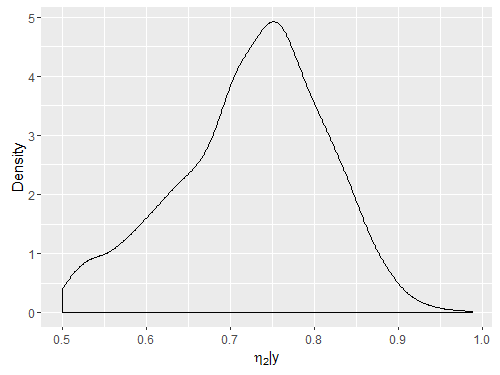
\includegraphics[width=\textwidth]{mainmatter/chapter_6_blood_donor/eta1.png}
        \caption{\label{fig : eta_blood_donor_1} Posterior $p(\eta_1|\boldsymbol{y})$}
	\end{subfigure}
	\begin{subfigure}[b]{0.4\textwidth}
		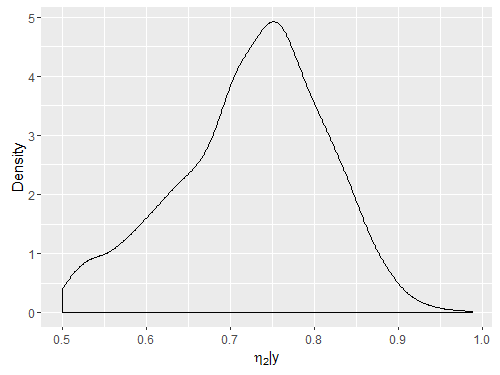
\includegraphics[width=\textwidth]{mainmatter/chapter_6_blood_donor/eta2.png}	
          \caption{\label{fig : eta_blood_donor_2}Posterior $p(\eta_2|\boldsymbol{y})$}
	\end{subfigure}	
	\caption{Posterior densities of the weight distribution for the components of the mixture of random effects for the blood donor data set.}
	\label{fig : eta_blood_donor}    
\end{figure} 

\begin{figure}[!htb]
\centering
\captionsetup{justification=centering}
\begin{subfigure}[b]{0.4\textwidth}
		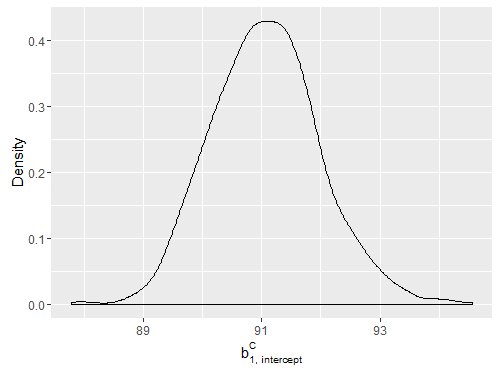
\includegraphics[width=\textwidth]{mainmatter/chapter_6_blood_donor/b11.png}
        \caption{\label{fig : mu_blood_donor_11}Posterior $p(b_\text{Intercept-1}^C|\boldsymbol{y})$}
	\end{subfigure}
	\begin{subfigure}[b]{0.4\textwidth}
		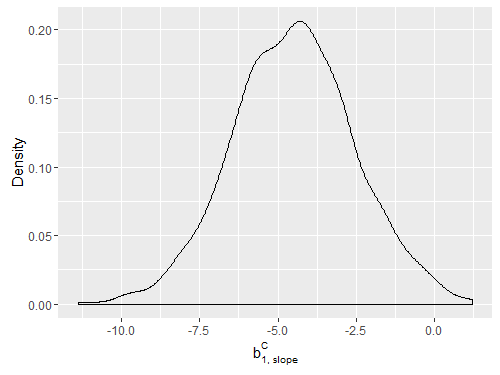
\includegraphics[width=\textwidth]{mainmatter/chapter_6_blood_donor/b12.png}	
          \caption{\label{fig : mu_blood_donor_12}Posterior $p(b_\text{Slope-1}^C|\boldsymbol{y})$}
	\end{subfigure}
	\begin{subfigure}[b]{0.4\textwidth}
		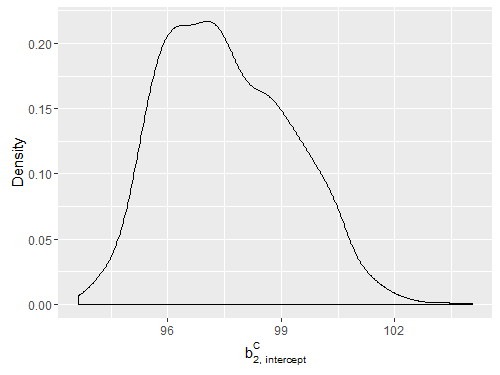
\includegraphics[width=\textwidth]{mainmatter/chapter_6_blood_donor/b21.png}	
          \caption{\label{fig : mu_blood_donor_21}Posterior $p(b_\text{Intercept-2}^C|\boldsymbol{y})$}
	\end{subfigure}	
	\begin{subfigure}[b]{0.4\textwidth}
		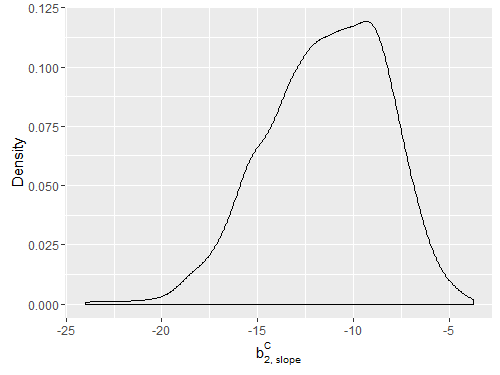
\includegraphics[width=\textwidth]{mainmatter/chapter_6_blood_donor/b22.png}	
          \caption{\label{fig : mu_blood_donor_22}Posterior $p(b_\text{Slope-2}^C|\boldsymbol{y})$}
	\end{subfigure}	
	\caption{Posterior densities of the location parameters for the components of the mixture of random effects for the blood donor data set.}
	\label{fig : mu_blood_donor}    
\end{figure} 

\begin{figure}[!htb]
\centering
\captionsetup{justification=centering}
\begin{subfigure}[b]{0.4\textwidth}
		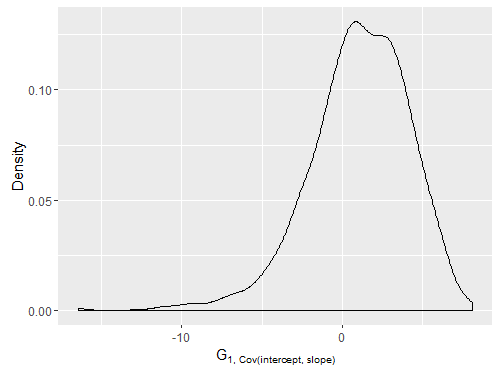
\includegraphics[width=\textwidth]{mainmatter/chapter_6_blood_donor/G11_1.png}
        \caption{\label{fig : cov_blood_donor_11_1}Posterior $p(\sigma^2_\text{Intercept-1}| \boldsymbol{y})$}
	\end{subfigure}
	\begin{subfigure}[b]{0.4\textwidth}
		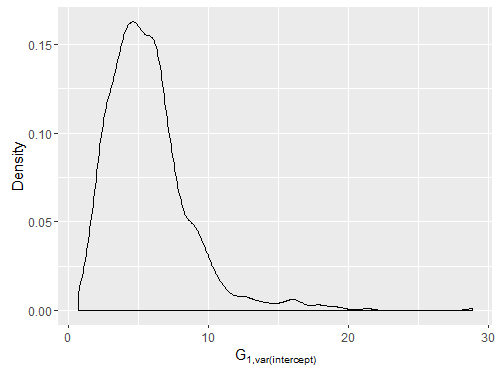
\includegraphics[width=\textwidth]{mainmatter/chapter_6_blood_donor/G12_1.png}	
          \caption{\label{fig : cov_blood_donor_12_1}Posterior $p(\sigma_{\text{Intercept-1}, \text{Slope-1}} | \boldsymbol{y})$}
	\end{subfigure}
	\begin{subfigure}[b]{0.4\textwidth}
		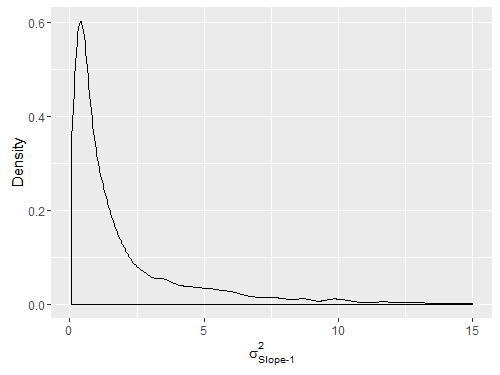
\includegraphics[width=\textwidth]{mainmatter/chapter_6_blood_donor/G22_1.png}	
          \caption{\label{fig : cov_blood_donor_22_1}Posterior $p(\sigma^2_\text{Slope-1}| \boldsymbol{y})$}
	\end{subfigure}	
	\begin{subfigure}[b]{0.4\textwidth}
		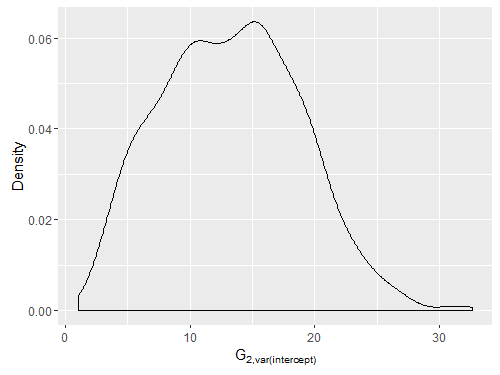
\includegraphics[width=\textwidth]{mainmatter/chapter_6_blood_donor/G11_2.png}
        \caption{\label{fig : cov_blood_donor_11_2}Posterior $p(\sigma^2_\text{Intercept-2}| \boldsymbol{y})$}
	\end{subfigure}
	\begin{subfigure}[b]{0.4\textwidth}
		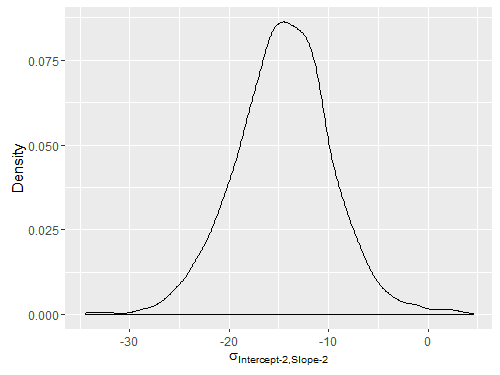
\includegraphics[width=\textwidth]{mainmatter/chapter_6_blood_donor/G12_2.png}	
          \caption{\label{fig : cov_blood_donor_12_2}Posterior $p(\sigma_{\text{Intercept-2}, \text{Slope-2}} | \boldsymbol{y})$}
	\end{subfigure}
	\begin{subfigure}[b]{0.4\textwidth}
		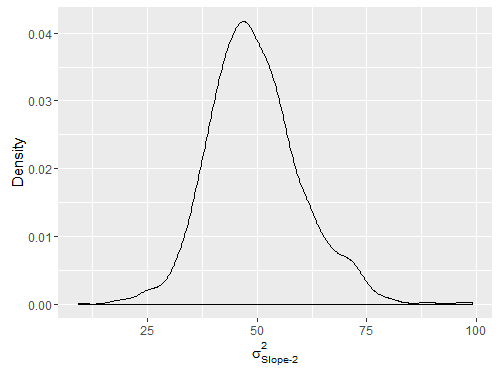
\includegraphics[width=\textwidth]{mainmatter/chapter_6_blood_donor/G22_2.png}	
          \caption{\label{fig : cov_blood_donor_22_2}Posterior $p(\sigma^2_\text{Slope-2}| \boldsymbol{y})$}
	\end{subfigure}	

	\caption{Posterior densities of the variance covariance parameters for the components of the mixture of random effects for the blood donor data set.}
	\label{fig : cov_blood_donor}    
\end{figure} 